\documentclass{beamer}

\mode<presentation>
{
  \usetheme{Hannover}

  \setbeamercovered{transparent}
}


\usepackage[english]{babel}
\usepackage[utf8]{inputenc}
\usepackage{graphicx} 
\usepackage{subcaption}
\usepackage{tikz} 



\title[Pulse Watcher]
{Java Advanced - Short Burst Project}

\subtitle
{Pulse Watcher}

\date{December 1, 2023}

\institute[Universities of Somewhere and Elsewhere]
{
  EHB\\
  Brussels}

\pgfdeclareimage[height=0.5cm]{university-logo}{ehb-logo.jpg}
\logo{\pgfuseimage{university-logo}}

% Delete this, if you do not want the table of contents to pop up at
% the beginning of each subsection:
\AtBeginSubsection[]
{
  \begin{frame}<beamer>{Outline}
    \tableofcontents[currentsection,currentsubsection]
  \end{frame}
}

\begin{document}

\begin{frame}
  \titlepage
\end{frame}


% Structuring a talk is a difficult task and the following structure
% may not be suitable. Here are some rules that apply for this
% solution: 

% - Exactly two or three sections (other than the summary).
% - At *most* three subsections per section.
% - Talk about 30s to 2min per frame. So there should be between about
%   15 and 30 frames, all told.

% - A conference audience is likely to know very little of what you
%   are going to talk about. So *simplify*!
% - In a 20min talk, getting the main ideas across is hard
%   enough. Leave out details, even if it means being less precise than
%   you think necessary.
% - If you omit details that are vital to the proof/implementation,
%   just say so once. Everybody will be happy with that.

\section{Context}

\subsection{Basic Problem}

\begin{frame}{Process monitoring}
  \begin{itemize}
  \item Programs fail
  \item Using \texttt{ssh} to check is inpracticle
  \item Central system \& standard
  \item Keeping an eye on usage
  \end{itemize}
\end{frame}

\begin{frame}{Features \& Technologies}
  This project uses:
  \begin{itemize}
  \item BackEnd
    \begin{itemize}
    \item Spring Boot
    \item Web Sockets
	\item Protocol Buffers
    \end{itemize}
  \item FrontEnd
    \begin{itemize}
    \item Vue.js
    \item Chart.js
    \end{itemize}
  \item Client
    \begin{itemize}
      \item Test Client in Go
      \item But could be {\bf anything}
    \end{itemize}
  \end{itemize}
\end{frame}

\subsection{Examples}

\begin{frame}{Grafana}

\begin{figure}
\begin{subfigure}[h]{0.65\linewidth}
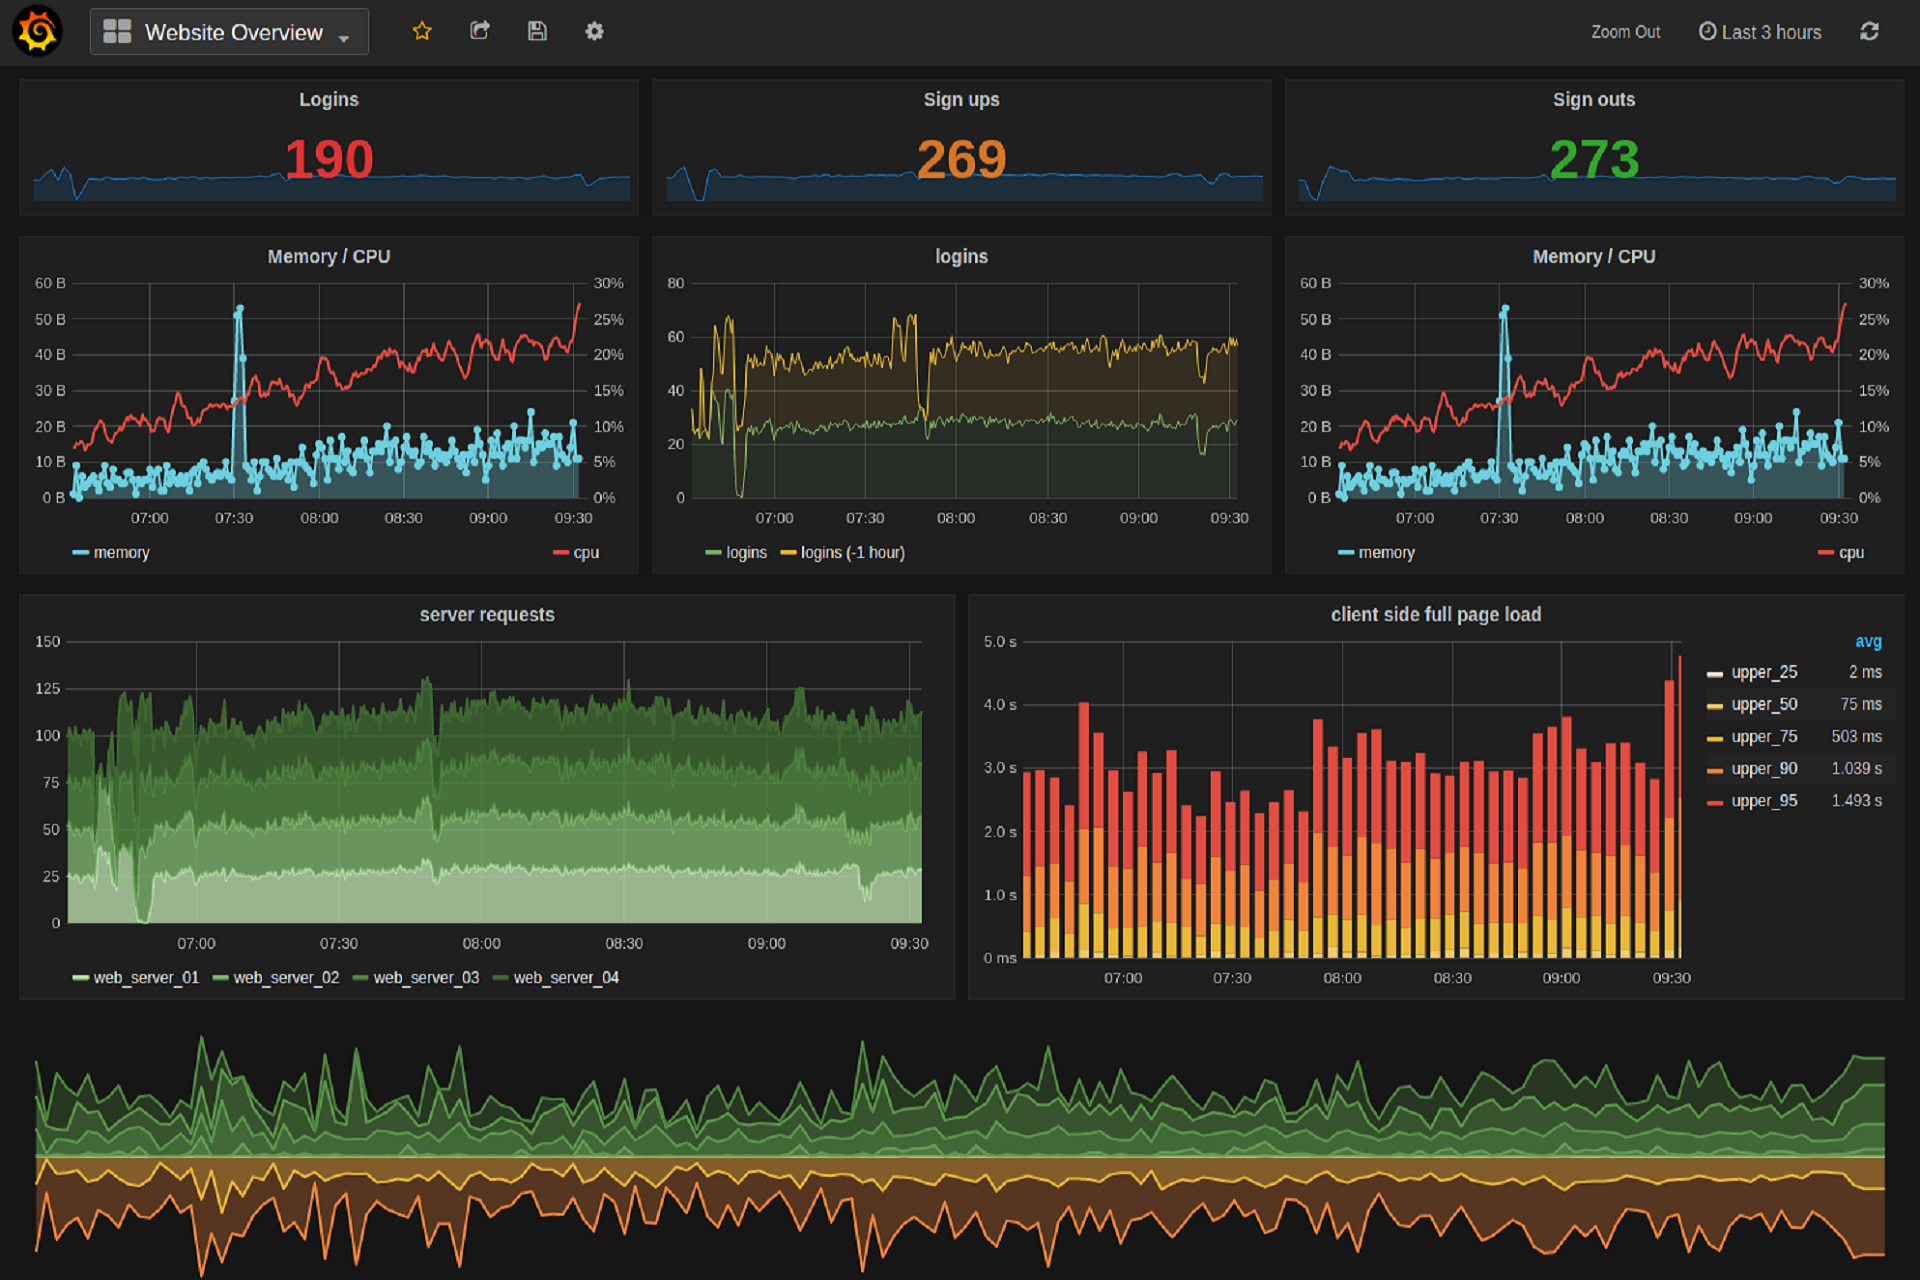
\includegraphics[width=\linewidth]{grafana.png}
\caption{Grafana Dashboard}
\end{subfigure}
\begin{subfigure}[h]{0.3\linewidth}

\includegraphics[width=\linewidth]{prometheus.png}
\caption{Prometheus logo}
\end{subfigure}
\end{figure}

\end{frame}

\section{Pulse Watcher}

\subsection{Demo}

\begin{frame}{Web UI}{Vue.js}

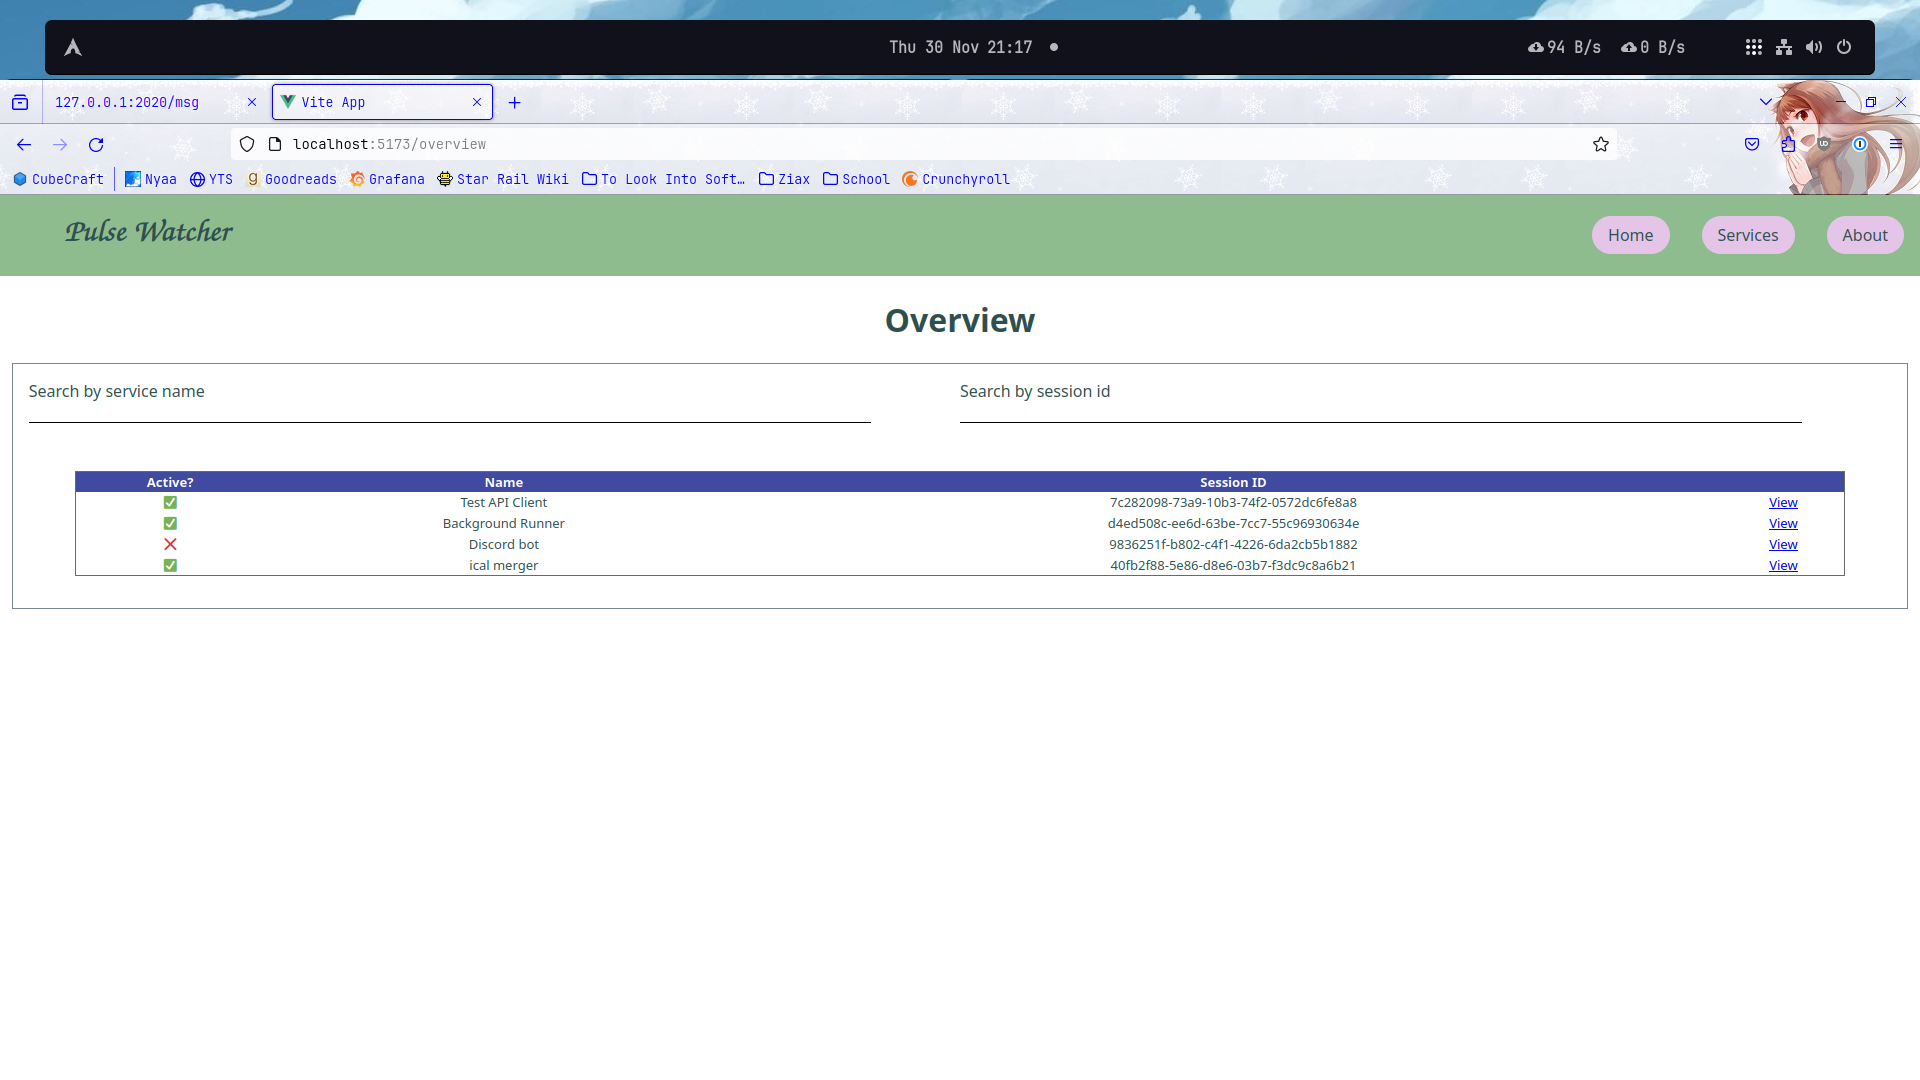
\includegraphics[width=\linewidth,keepaspectratio]{web_ui_1.png}

\end{frame}

\begin{frame}{Web UI}{Vue.js}

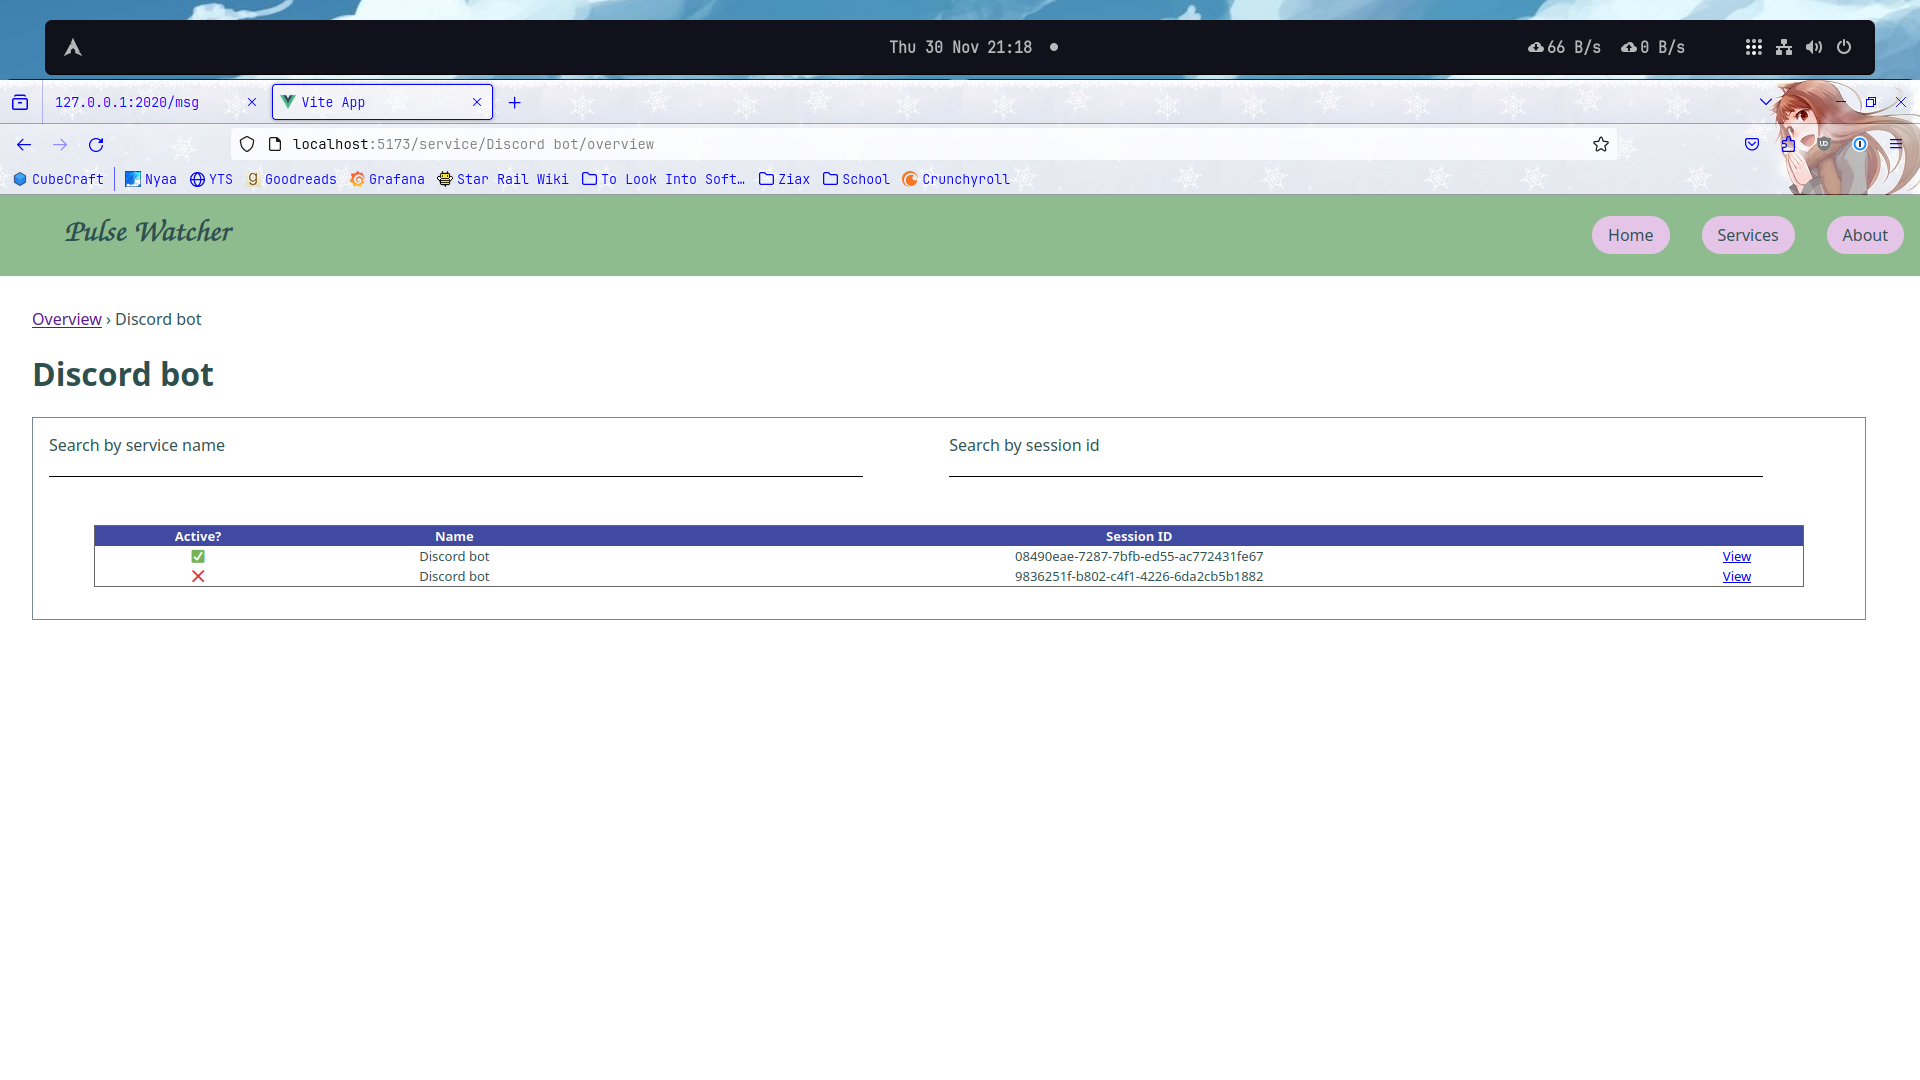
\includegraphics[width=\linewidth,keepaspectratio]{web_ui_2.png}

\end{frame}

\begin{frame}{Web UI}{Vue.js}

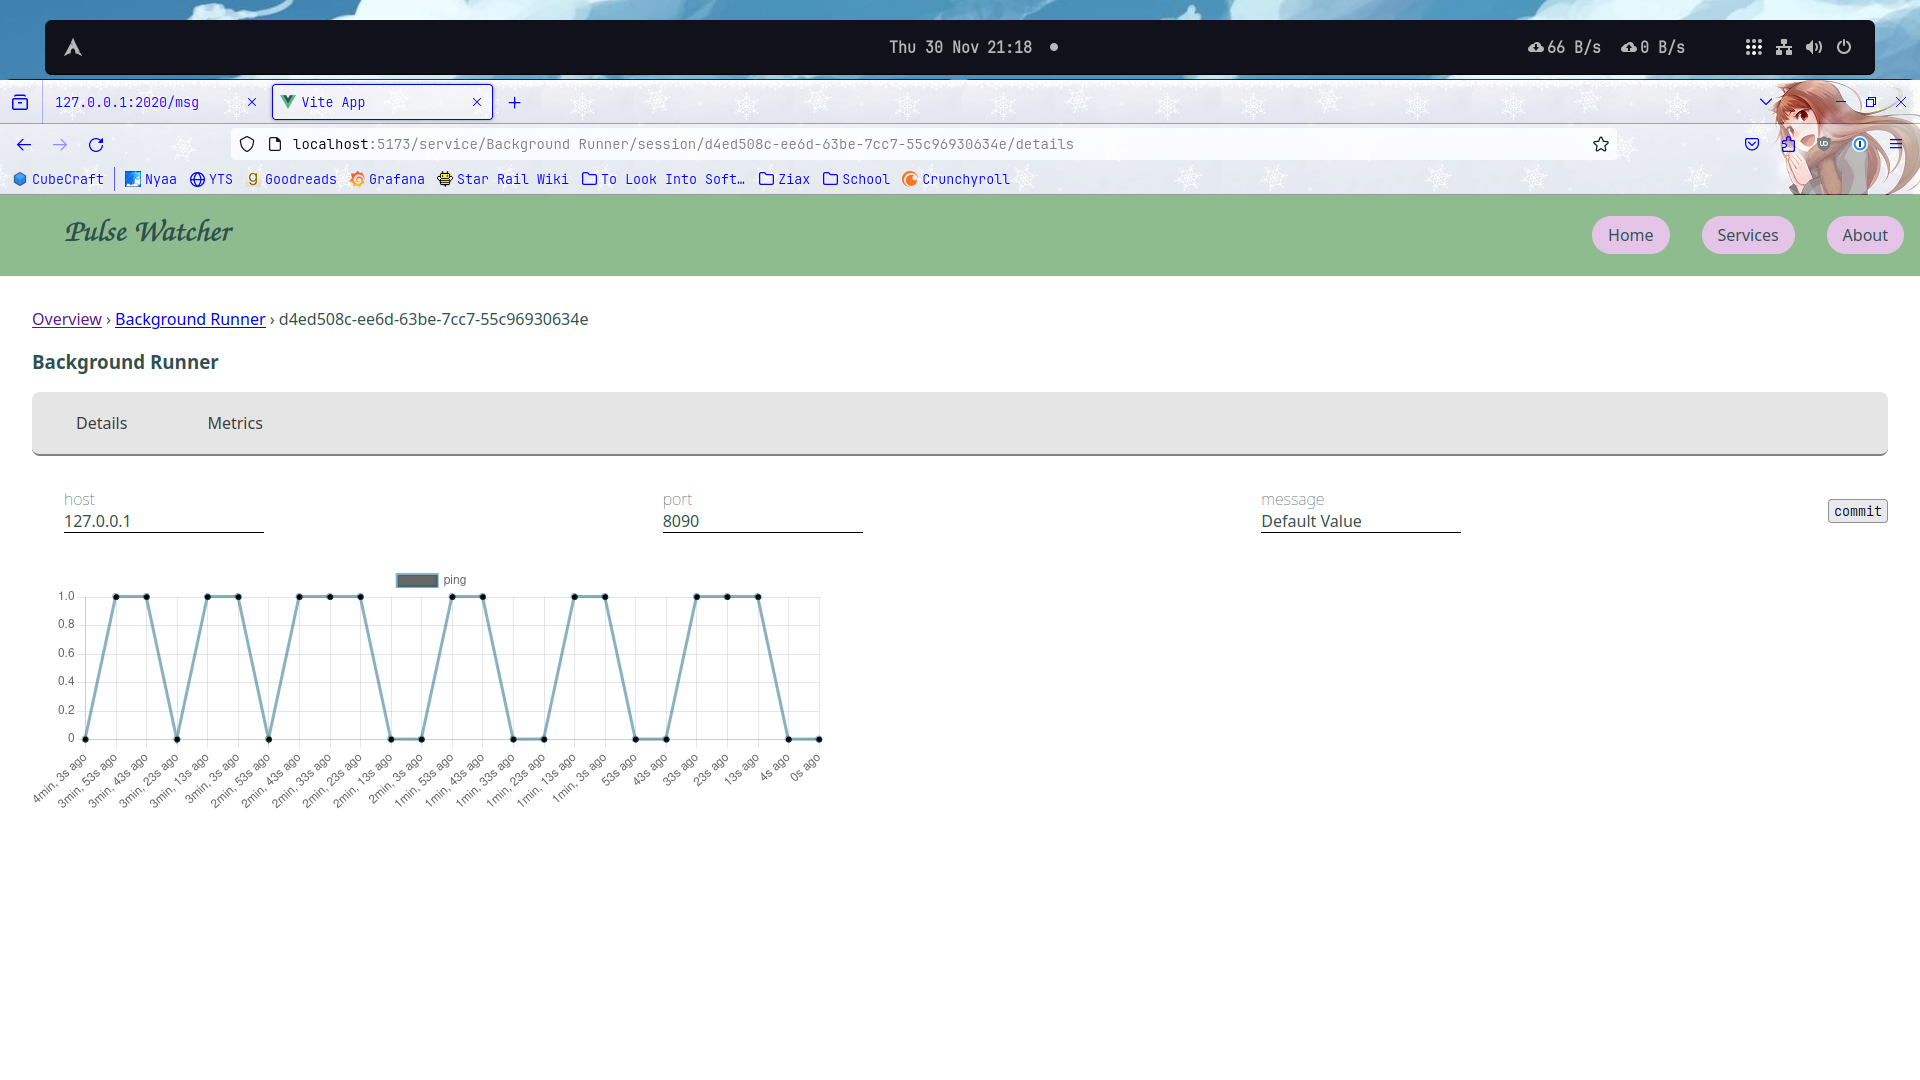
\includegraphics[width=\linewidth,keepaspectratio]{web_ui_3.png}

\end{frame}

\begin{frame}{Web UI}{Vue.js}

\url{https://youtu.be/TcF3HiDM8kI}

\end{frame}


\subsection{Implementation}

\begin{frame}{Backend}{Springboot}

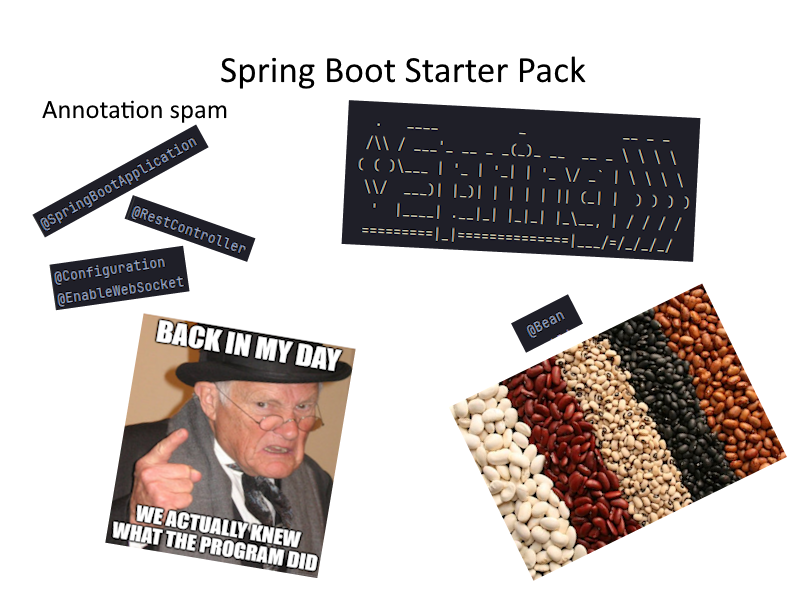
\includegraphics[width=\linewidth,keepaspectratio]{spring_boot_meme.png}


\end{frame}

\begin{frame}{Backend}{Server $<$-$>$ Client Web Socket}

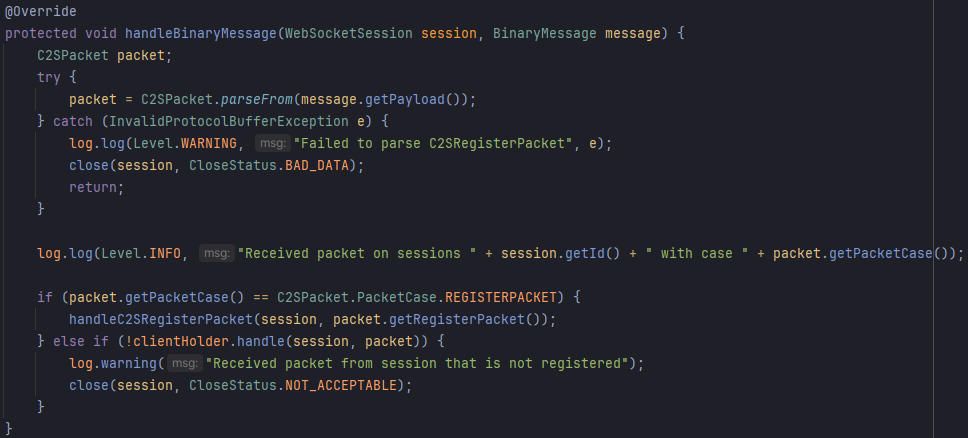
\includegraphics[width=\linewidth,keepaspectratio]{code_snippet.png}

\end{frame}

\begin{frame}{Backend}{Server $<$-$>$ Client Web Socket}

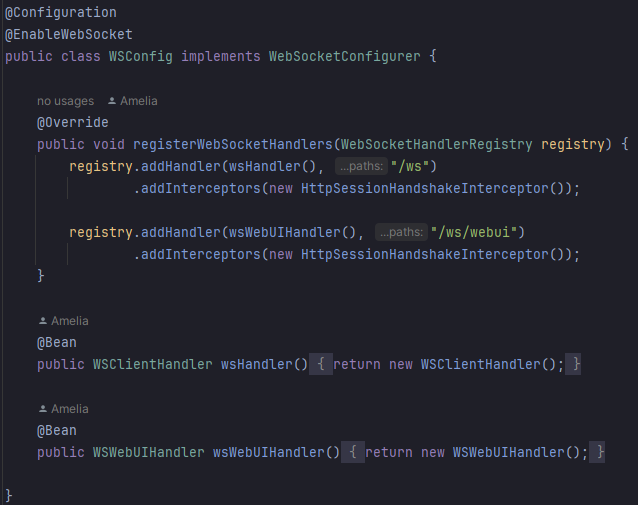
\includegraphics[width=\linewidth,keepaspectratio,height=0.7\textwidth]{code_snippet_2.png}

\end{frame}

\begin{frame}{Backend}{Life cycle}

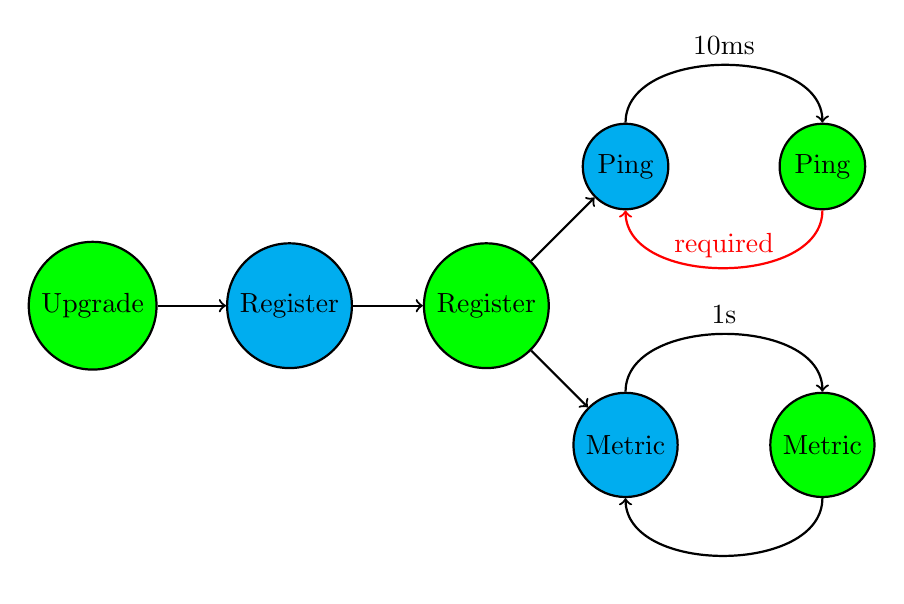
\begin{tikzpicture}[
node distance={25mm},
thick,
client/.style = {draw, circle, fill=green},
server/.style ={draw, circle, fill=cyan} ] 
\node[client] (1) {Upgrade};
\node[server] (2) [right of=1] {Register};
\node[client] (3) [right of=2] {Register};

\node[server] (4) [above right of=3] {Ping};
\node[client] (5) [right of=4] {Ping};

\node[server] (6) [below right of=3] {Metric};
\node[client] (7) [right of=6] {Metric};

\draw[->] (1) -- (2);
\draw[->] (2) -- (3);
\draw[->] (3) -- (4);
\draw[->] (3) -- (6);
\draw[->] (4) to [out=90, in=90] node[midway, above] {10ms} (5);
\draw[->,color=red] (5) to [out=270, in=270] node[midway,above] {required} (4);
\draw[->] (6) to [out=90, in=90] node[midway, above] {1s} (7);
\draw[->] (7) to [out=270, in=270] (6);

\end{tikzpicture}

\end{frame}

\begin{frame}{API}{Protobuffers}
\begin{figure}
\begin{subfigure}[h]{0.45\linewidth}
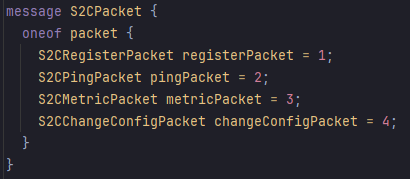
\includegraphics[width=\linewidth]{code_snippet_3.png}
\caption{{\bf S}erver to {\bf C}lient Packet}
\end{subfigure}
\begin{subfigure}[h]{0.45\linewidth}
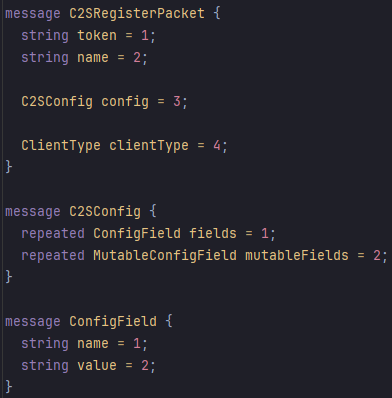
\includegraphics[width=\linewidth]{code_snippet_4.png}
\caption{C2S Register Packet}
\end{subfigure}
\end{figure}
\end{frame}

\begin{frame}{API}{Protobuffers}

\begin{itemize}
\item Actual Types
\item Not language depended
\item Smart compiler
\end{itemize}
{\tiny protoc -I=./ --java\_out=./src/main/java/ --go\_out=./test-client/  packets.proto}

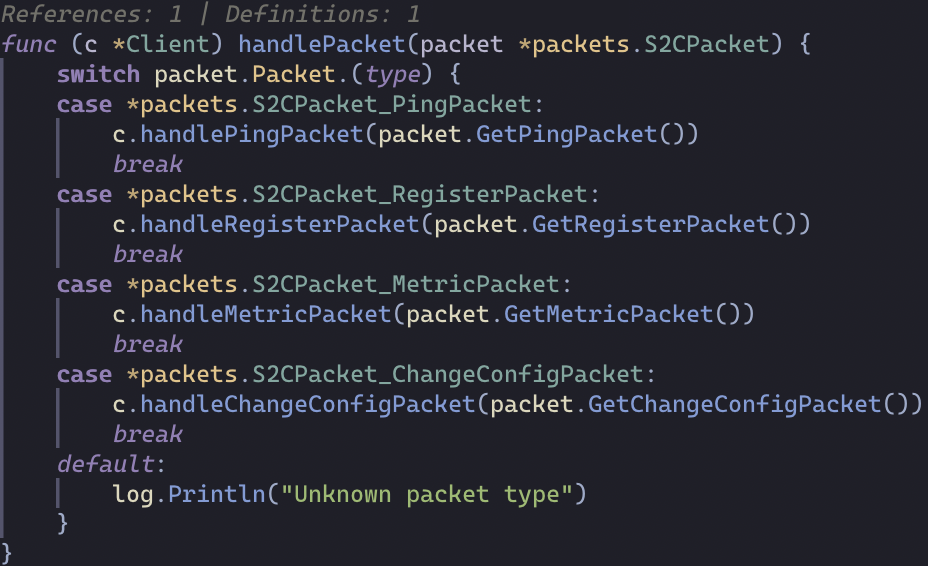
\includegraphics[width=\linewidth,height=0.5\textwidth]{code_snippet_5.png}
\end{frame}


\section*{Summary}

\begin{frame}{Summary}
  \begin{itemize}
  \item Front end development \alert{is a pain}.
  \item Google's \alert{protocol buffers} are wicked cool.
  \item Spring Boot is impressive but, \alert{a black box}.
  \end{itemize}
\end{frame}



% All of the following is optional and typically not needed. 
\appendix
\section<presentation>*{\appendixname}
\subsection<presentation>*{References \& Documentation}

\begin{frame}[allowframebreaks]
  \frametitle<presentation>{Bibliography}
    
  \begin{thebibliography}{10}
  
  \setbeamertemplate{bibliography item}[online]	

  \bibitem{protobuf-docs}
    Google LLC
    \newblock {\em Protocol Buffers - \url{https://protobuf.dev/}}.
    \newblock \textcopyright 2023
 
  
  \bibitem{vue-docs}
    Evan You
    \newblock {\em Vue.js - \url{https://vuejs.org/}}
    \newblock \textcopyright 2104-2023
    
    \bibitem{spring-boot}
    VMware Tanzu
    \newblock {\em Spring Boot - \url{https://spring.io/}}
    \newblock \textcopyright 2005-2023
  \end{thebibliography}
\end{frame}

\end{document}


